\documentclass[12pt]{beamer}

\usepackage[utf8]{inputenc}
\usepackage{amsmath}
\usepackage{amssymb} 
\usepackage{amsmath}
\usepackage{amsthm}
\usepackage{algorithm}
\usepackage{algorithmicx}
\usepackage[noend]{algpseudocode}
\usepackage{float}
\newcommand{\norm}[1]{\left\lVert#1\right\rVert}
\newtheorem{proposition}{Proposición}
\usepackage{graphicx}
\usepackage{tikz}
\usetikzlibrary{positioning,fit}
\usepackage{caption}
\usepackage{subcaption}

\title{Métodos iterativos para la solución de problemas inversos discretos}

\author{Jazmín Rivas, Kevin Luna, Fausto Martinez, Aaron Klarreich}
\date{Martes 17 de diciembre}

\begin{document}
	
	\begin{frame}
		\titlepage
	\end{frame}
	
	\section{Introducción} 
	% En esta sección va a ir Motivación, Métodos iterativos (definiciones, formula, Jacobi/G-S, etc).
	
	\begin{frame}{Motivación}
		
		\ En este texto se pretende estudiar el problema de enfoque de imágenes. A partir de una imagen borrosa con ruido y una matriz de desenfoque, nuestro objetivo es encontrar nuestra imagen original utilizando su versión borrosa. Este problema se puede formular a través de un sistema lineal $Ax = b$, donde $A$ es la matriz de desenfoque, $b$ es el ruido y $x$ es la imagen a restaurar. Debido a su mal condicionamiento, nos interesan los métodos de regularización para la reconstrucción de las mismas. En particular, nos interesaremos por los métodos de regularización de Krylov. Estos métodos están basados en procesos de proyección sobre un tipo de subespacios muy particulares, de los cuales el método toma el nombre. Este capítulo servirá de introducción a la estructura general de esta clase de métodos.
		
	\end{frame}
	
	\begin{frame}{Métodos Iterativos}
		
		\ Ante las limitaciones que traen los métodos de resolucón de problemas del estilo $Ax = b$, los métodos iterativos buscan superar los problemas de estos métodos para producir soluciones a estos sistemas. \\
		\ Si consideramos $A = M-N$, tenemos que: $$(M-N)x = b$$ o bien: $$x = M^{-1}(b+Nx)$$ lo que nos da la fórmula recursiva $$x_{n+1} = M^{-1}(b+Nx_n)$$
		
	\end{frame}
	
	\begin{frame}{Métodos Estandar}
		
		\ Partiendo de la forma $x_{n+1} = M^{-1}(b+Nx_n)$, si tomamos $N = M-A$ tenemos que: $$x_{n+1}=M^{-1}(b+(M-A)x_{n})=M^{-1}b+x_n-M^{-1}Ax_n$$ luego, $$x_{n+1}=x_n+M^{-1}(b-Ax_n)$$ La cual es la fórmula general para cualquier método iterativo. Más aún, si descomponemos a $A$ como $A = L+D+U$ como sus partes \textit{lower}, \textit{diagonal} y \textit{upper} podemos definir los métodos iterativos más comunes.
		
	\end{frame}
	
	\begin{frame}{Método de Jacobi}
		
		\ Como $A = L+D+U$, tenemos que $$Ax=b \iff Dx=-(L+U)x+b$$ con lo que podemos escribir la forma recursiva como: $$Dx_{n+1}=-(L+U)x_n+b$$ y esto nos dice que: $$x_{n+1}=-D^{-1}(L+U)x_n+D^{-1}b$$ la cual es la iteración del método de Jacobi.
		
	\end{frame}
	
	\begin{frame}{Método de Gauss-Seidel}
		
		\ De la misma forma, podemos decir que $$Ax=b \iff (L+D)x=-Ux+b$$ y nos induce la forma recurisva $$(L+D)x_{n+1}=-Ux_n+b$$ que podemos reescribir como la iteración del método de Gauss-Seidel: $$x_{n+1}=-(L+U)^{-1}Ux_n+(L+U)^{-1}b$$ \\
		\ En general, podemos decir que las iteraciones de los métodos vienen dadas por $x_{n+1}=Bx_n+C$, y en el caso de Jacobi, $B_J=-D^{-1}(L+U)$ y $C_J=D^{-1}b$ y para Gauss-Seidel $B_{GS}=-(L+U)^{-1}U$ y $C_{GS}=(L+U)^{-1}b$.
		
	\end{frame}
	
	\section{Teoría}
	% Acá va a ir todo lo de Krylov, métodos de proyección, Arnoldi, GMRES, LSQR, Tikhonov, etc. 
	
	\begin{frame}{Métodos de Krylov}
		
		\begin{definition}
			Dada $A$ una matriz y $v, Av, \dots , A^{m-1}v \in \mathbb{C}^m$ vectores linealmente independientes, llamamos subespacio de Krylov de dimensión $m$ a: $$\mathcal{K}_{m}(A, v) = \langle v, Av, \ldots, A^{m-1}v \rangle$$
		\end{definition} 
		Los métodos de Krylov son métodos iterativos que utilizan subespacios de Krylov que, dado $x_0$ una aproximación inicial de la solución del sistema, se define el subespacio $\mathcal{K}_{m}(A, r_0)$, con $r_0=b-Ax_0$.
		
	\end{frame}
	
	\begin{frame}{Motivación del Método}
		
		\ Sea $x_{true}=A^{-1}b$ y $x_0$ una aproximación inicial para el método, resolver el sistema original es equivalente a resolver $Az=r_0$ si $z=x_{true}-x_0$. Sea $p(x)$ el polinomio de menor grado $i$ tal que $p(A)r_0=0$. Por el teorema de Cayley-Hamilton, tenemos que $i\leq n$. Entonces tenemos que: $$p(A)=a_0+Aa_1+\dots+a_{i-1}A^{i-1}+a_iA^i=0$$ 
		
	\end{frame}
	
	\begin{frame}{Motivación del Método}
		
		Por lo que vale que $$A^{-1}a_0=-(a_1I+a_2A+\dots+a_{i-1}A^{i-2}+a_iA^{i-1})$$ Y si multiplicamos por $r_0$ tenemos que: $$z=A^{-1}r_0=-\frac{1}{a_0}(a_1I+a_2A+\dots+a_{i-1}A^{i-2}+a_iA^{i-1})r_0$$ Por lo que $$z\in \langle r_0,Ar_0,\dots,A^{i-1}r_0 \rangle = \mathcal{K}_{m}(A, r_0)$$ o bien, $$x_{true} \in x_0 + \mathcal{K}_{m}(A, r_0).$$
		
	\end{frame}
	
	\begin{frame}{Métodos de Proyección}
		
		\ Como $x_{true} \in x_0 + \mathcal{K}_{m}(A, r_0)$, naturalmente la solución $x_n$ puede estar dada por $$x_n = x_0 + y_n, \quad  y_n \in \mathcal{K}_n(A, r_0).$$ Dado $x_0 \in \mathbb{C}^n$ una aproximación inicial a nuesta solución y $r_0 := b - Ax_0$, definimos al residuo en la iteración $n$ está dado por: $$r_n := b - Ax_n = b - A(x_0 + y_n) = r_0 - Ay_n, \quad r_n\in \ \mathcal{K}_{n+1}(A, r_0).$$ Veamos algunos enfoques para determinar $x_n$ de manera óptima.
		
	\end{frame}
	
	\begin{frame}{Enfoque de Ritz-Galerkin y Petrov-Galerkin}
		
		\begin{flushleft}
			\textbf{Enfoque de Ritz-Galerkin}
		\end{flushleft} 
		Para este enfoque, necestimaos imponer una reestricción en cuanto a la noción de ortgonalidad de la siguiente manera para cada $n \in \mathbb{N}$: $$r_n \perp \mathcal{K}_{n}(A, r_0)$$
		
		\begin{flushleft}
			\textbf{Enfoque de Petrov-Galerkin}
		\end{flushleft}
		\ Aquí vamos a pedir que el residuo sea ortogonal a un subespacio $\mathcal{L} \subset \mathbb{C}^{n}$ de dimensión $n$, es decir, 	$$r_n \perp \mathcal{L}_n, \quad dim(\mathcal{L}_n) = n$$
	\end{frame}
	
	\begin{frame}{Método de Arnoldi}
		
		\ Sea $V_i$ la matriz de tamaño $n\times i$ con $v_1, ..., v_i$ como columnas, $H_i$ la matriz de Hessenberg de tamaño $(i+1)\times i$ cuyos elementos no nulos son los $h_{ij}$ descritos en el algoritmo de Arnoldi, entonces se verifica que: $$AV_j=V_{j+1}H_i$$
		
		
		
	\end{frame}
	
	\begin{frame}
		
		\begin{algorithm}[H]
			\caption{Algoritmo de Arnoldi}\label{algorithm_1}
			\begin{algorithmic}[1]
				\State Comencemos con $v_1=\frac{v}{\norm{v}}$
				\For{$j \in \{1, 2, \dots, i\}$}
				
				\State Computamos $h_{ij} = v_i^TAv_j$ para $i \in \{1, 2, \dots, j\}$
				\State $w_j = Av_j - \sum_{i=1}^j h_{ij} v_i$
				\State $h_{j+1,j} = \|w_j\|_2$
				\If{$h_{j+1,j} = 0$}
				
				\State Stop
				\EndIf
				\EndFor
				\State $v_{j+1} = w_j / h_{j+1,j}$
			\end{algorithmic}
		\end{algorithm}   
		
	\end{frame}
	
	\begin{frame}{GMRES}
		
		\ GMRES (Generalized Minimal Residual Method) busca minimizar $J(y)=||b-Ax||_2$ a través de sus componentes ortonormales, minimizando en cada paso los vectores residuales. \\
		\ Sea $x_0$ una aproximación inicial, tenemos que para todo $x_i\in\mathcal{K}_m+x_0$ vale que $$x=x_0+V_my$$ donde $V_m$ es la misma matriz definida en el método de Arnoldi, e $y$ es un vector de tamaño $m$.
		
	\end{frame}
	
	\begin{frame}{GMRES}
		
		Sean $\beta = ||r_0||_2$ y $v_1=\frac{r_0}{||r_0||_2}$, y teniendo en cuenta la igualdad en el metodo de Arnoldi, podemos reescribir el problema a minimizar como:
		\begin{equation*}
			\begin{split}
				b-Ax&=b-A(x_0+V_my)\\
				`    &= r_0-AV_my\\
				&= \beta v_1-V_{m+1}H_my\\
				&= V_{m+1}(\beta e_1 - H_my)
			\end{split}
		\end{equation*}
		luego, 
		\begin{equation*}
			\begin{split}
				J(y)&=||b-Ax_i||_2\\
				&=||V_{m+1}(\beta e_1 - H_my_m)||_2    
			\end{split}
		\end{equation*}
		y como los vectores columna de $V_{m+1}$ son ortonormales, entonces:
		$$J(y)=||\beta e_1 - H_my||_2$$
		
	\end{frame}
	
	\begin{frame}
		
		\begin{algorithm}[H]
			\caption{Algoritmo GMRES}
			\begin{algorithmic}[1]
				\State \textbf{Dada} $\mathbf{A} \in \mathbb{R}^{n \times n}$, $\mathbf{b} \in \mathbb{R}^n$, $\mathbf{x}^{(0)}$, calcular $\mathbf{r}^{(0)} = \mathbf{b} - \mathbf{A} \mathbf{x}^{(0)}$
				\State $\mathbf{v}_1 = \frac{\mathbf{r}^{(0)}}{\|\mathbf{r}^{(0)}\|}$
				\For{$k = 1, 2, \dots, m$}
				\State Calcular $\mathbf{w_k} = \mathbf{A} \mathbf{v}_k$
				\For{$j = 1, \dots, k$}
				\State $h_{jk} = \mathbf{w}^T \mathbf{v}_j$
				\State $\mathbf{w_k} := \mathbf{w_k} - h_{jk} \mathbf{v}_j$
				\EndFor
				\State $h_{k+1,k} = \|\mathbf{w_k}\|$
				\If{$h_{k+1,k} \neq 0$}
				\State $\mathbf{v}_{k+1} = \frac{\mathbf{w_k}}{h_{k+1,k}}$
				\EndIf
				\EndFor
				\State Resolver el problema de mínimos cuadrados $\min_y \|\beta \mathbf{e}_1 - \mathbf{H}_k y\|_2$
				\State Actualizar la solución: $\mathbf{x}^{(k)} = \mathbf{x}^{(0)} + \mathbf{V}_k y$
				\If{$\|\mathbf{r}^{(k)}\| <$ tolerancia}
				\State Romper el ciclo
				\EndIf
			\end{algorithmic}
		\end{algorithm}
		
	\end{frame}
	
	\begin{frame}{Regularización de Tikhonov}
		
		\ La regularización es una técnica que busca sistemas lineales mal condicionados agregando un término regularizante. Tikhonov en particular busca resolver $$\min_{x} \left( \| \mathbf{A}x - \mathbf{b} \|_2^2 + \lambda \| \mathbf{x} \|_2^2 \right)$$ con $\lambda > 0$ el parámetro regularizante. Si consideramos $\phi(x) = \|Ax - b\|^2 + \lambda \|x\|^2$, tenemos que: \[
		\nabla \phi(x) = 2A^T(Ax - b) + 2\lambda x = 0 \iff 
		\boxed{(A^TA + \lambda \mathrm{Id})x = A^Tb}
		\]
		
	\end{frame}
	
	\begin{frame}{Regularización de Tikhonov generalizada}
		\ En general, se suele pedir que la solución minimice cierta cantidad 
		\[
		\Omega(x) = \| L(x) \|_2
		\] con $L$ un operador que bien puede ser la identidad o el operador de derivación. Si además conocemos un estimador inicial de la solución $x^*$, $$\Omega(x) = \| L(x - x^*) \|^2.$$ Y en definitiva queremos encontrar $$\min \left( \| \mathbf{A}x - \mathbf{b} \|_2^2 + \lambda \| \mathbf{L(x - x^*)} \|_2^2 \right)$$
		
		
	\end{frame}
	
	\begin{frame}{Descomposición SVD}
		
		\ Sea $A \in \mathbb{R}^{m \times n}$, la descomposición SVD nos permite escrbrir a $A$ como: $$A = U \Sigma V^T = \sum_{i=1}^{n} \sigma_i u_i v_i^T$$
		donde:
		
		\begin{itemize}
			\item \( U \) es una matriz cuyas columnas son los vectores propios ortonormales de \( A A^T \).
			\item \( \Sigma \) es una matriz diagonal con los valores singulares de \( A \) en la diagonal.
			\item \( V^T \) es la transpuesta de una matriz cuyas filas son los vectores propios ortonormales de \( A^T A \).
		\end{itemize}
		
	\end{frame}
	
	\begin{frame}{Curva L}
		
		\ Una forma de hallar el valor regularizador es la Curva L, que consiste en graficar la relación entre la norma del residuo y la de la solución: $$L(\lambda) := \{(\phi (\| x_\lambda  \|^2), \phi (\| \mathbf{A}x_\lambda - \mathbf{b} \|^2) ): \lambda > 0\}$$ con $\phi$ una función monótona creciente, generalmente $\phi(t) = \log(t)$ o $\phi(t) = t$.
		
		\begin{proposition}
			Sean $q(\lambda) = \phi (\| x_\lambda  \|^2)$ y $s(\lambda) = \phi (\| \mathbf{A}x_\lambda - \mathbf{b} \|^2 )$, con $L = \mathrm{Id}$ y $\phi$ una función diferenciable y monótona creciente. Entonces $q(\lambda)$ es una función decreciente y $s(\lambda)$ es creciente en función de $\lambda$.
		\end{proposition}
		
	\end{frame}
	
	
	\section{Implementación}
	% Acá va a ir todo lo de Faus, código, implementaciones, ejemplos, bla bla
	
	\begin{frame}{Ejemplo}
		
		\ Con todo esto en mente, ahora implementemoslo a un ejemplo práctico. Consideremos la siguiente imágen generada de un mate:
		\begin{figure}[htp]
			\centering
			
\includegraphics[width=3.5cm]{Imagenes/Imagenes/x_true.png}
		\end{figure}
		
		\ A lo largo del ejemplo veremos cómo reconstruir esto si agregamos ruido con las herramientas que aprendimos.
		
	\end{frame}
	
	\begin{frame}{Operador de Desenfoque}
		
		Primero veamos cómo la operador de desenfoque $\mathbf A$ afecta a un punto:
		
		\begin{figure}[htp]
			\centering
			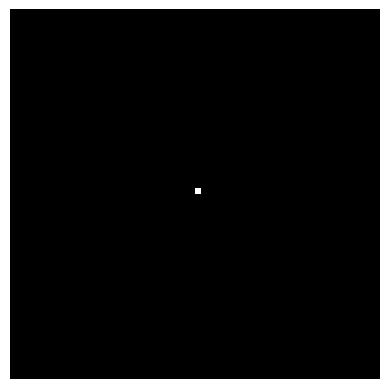
\includegraphics[width=3cm]{Imagenes/Imagenes/y_pixel.png}
			\qquad\tikz[baseline=-\baselineskip]\draw[ultra thick,->] (0,0) -- ++ (1,0);\qquad % NO PUDE ENCONTRAR COMO CENTRARLA
			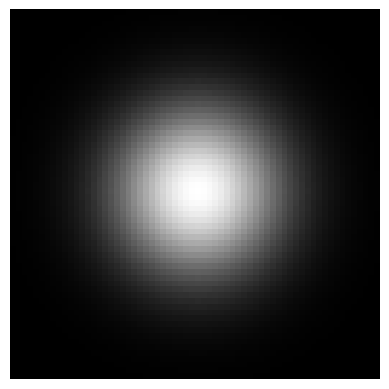
\includegraphics[width=3cm]{Imagenes/Imagenes/Ay_pixel.png}
			\label{fig:mate}
		\end{figure}
		
		
	\end{frame}
	
	\begin{frame}{Construcción del problema}
		
		\ Nosotros vamos a tener un $\mathbf b$ que representaría nuestra imágen ya desenfocada. A partir de él, vamos a reconstruir a $\mathbf x_{true}$ nuestra imágen original. Nuestro punto de partida sería $\mathbf b_{true}=\mathbf A \mathbf x_{true}$.
		
		\begin{figure}[htp]
			\centering
			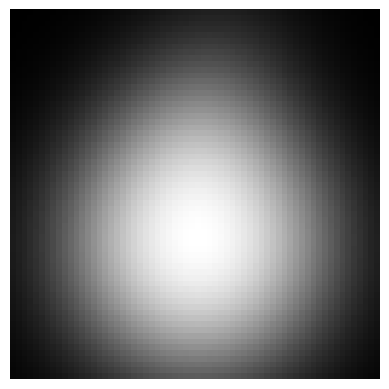
\includegraphics[width=3.5cm]{Imagenes/Imagenes/b_true.png}
			\label{fig:mate}
		\end{figure}
		
	\end{frame}
	
	\begin{frame}{Tipos de ruido}
		
		\ Estos son los tipos más normales de ruido que podríamos encontrarnos, aunque nosotros trabajaremos con un ruido Gaussiano.
		
		\begin{figure}
			\centering
			\begin{minipage}{.5\textwidth}
				\centering
				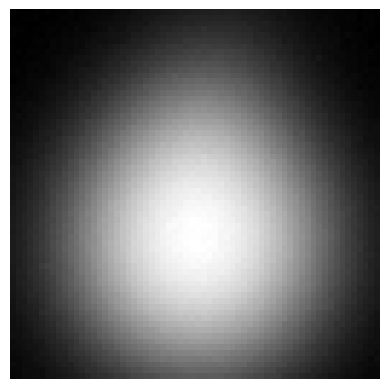
\includegraphics[width=.4\linewidth]{Imagenes/Imagenes/mate_Gauss.png}
				\captionof{figure}{Ruido Gaussiano}
			\end{minipage}%
			\begin{minipage}{.5\textwidth}
				\centering
				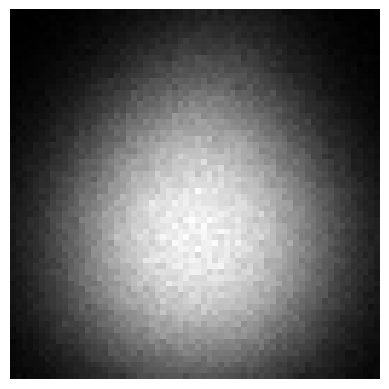
\includegraphics[width=.4\linewidth]{Imagenes/Imagenes/mate_Poisson.png}
				\captionof{figure}{Ruido Poisson}
			\end{minipage}
			\begin{minipage}{.5\textwidth}
				\centering
				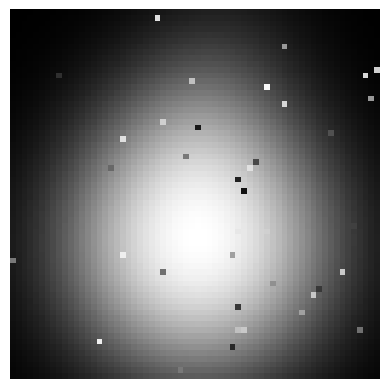
\includegraphics[width=.4\linewidth]{Imagenes/Imagenes/mate_saltpepper.png}
				\captionof{figure}{Ruido Salt \& Pepper}
			\end{minipage}
		\end{figure}
		
	\end{frame}
	
	\begin{frame}{Regularización}
		
		\ La solución directa del sistema $\mathbf Ax=b$ no es una buena idea, ya que nos devuelve esto:
		
		\begin{figure}[htp]
			\centering
			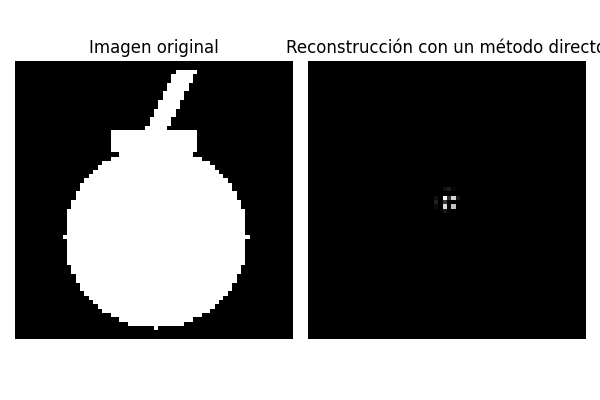
\includegraphics[width=9cm]{Imagenes/Imagenes/mate_metodoDirecto.png}
		\end{figure}
		
		\ Por eso recurrimos a métodos de regularización que salven este problema.
		
	\end{frame}
	
	\begin{frame}{GMRES}
		
		\ Si utilizamos GMRES para poder conseguir soluciones iterativamente y conseguimos pararlo antes que la solución se contamine demasiado de ruido conseguimos esto:
		
		\begin{figure}[htp]
			\centering
			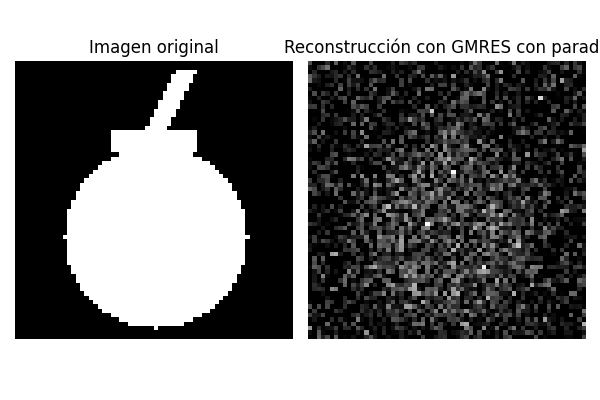
\includegraphics[width=9cm]{Imagenes/Imagenes/mate_GMRES.png}
		\end{figure}
		
	\end{frame}
	
	\begin{frame}{Tikhonov}
		
		\ Otra idea que puede surgir es usar Tikhonov, que después de trabajar la solución podemos obtener esto:
		
		\begin{figure}[htp]
			\centering
			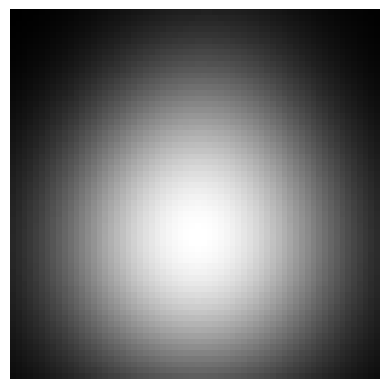
\includegraphics[width=4cm]{Imagenes/Imagenes/mate_tikh_lambda_arbitrario.png}
		\end{figure}
		
		\ Pero esto se puede mejorar.
		
	\end{frame}
	
	\begin{frame}{Elección de $\lambda$}
		
		\ Como ya vimos, la Curva L puede ser un buen método para encontrar un $\lambda$ apropiado, comparando $\|\mathbf{Ax}^{\rm reg} - \mathbf{b}\|$ vs $\|\mathbf{x}^{\rm reg}\|$. Esto nos lleva al siguiente resultado:
		
		\begin{figure}[htp]
			\centering
			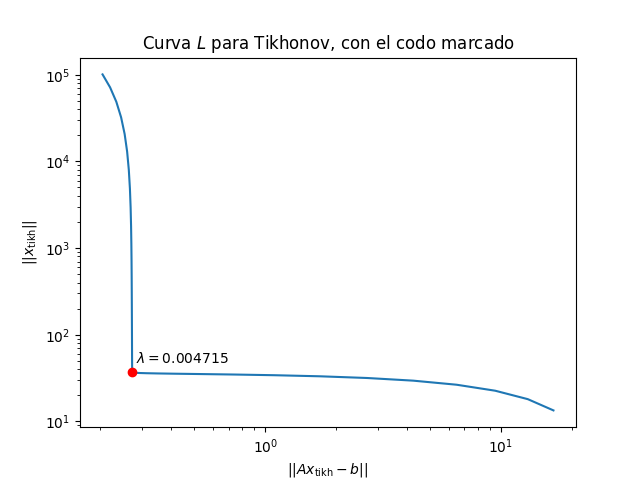
\includegraphics[width=8.5cm]{Imagenes/Imagenes/L_curve_tikh_codo.png}
		\end{figure}
		
	\end{frame}
	
	\begin{frame}{Tikhonov}
		
		\ Ahora con una elección de $\lambda$ óptima, con Tikhonov podemos lograr esto:
		
		\begin{figure}[htp]
			\centering
			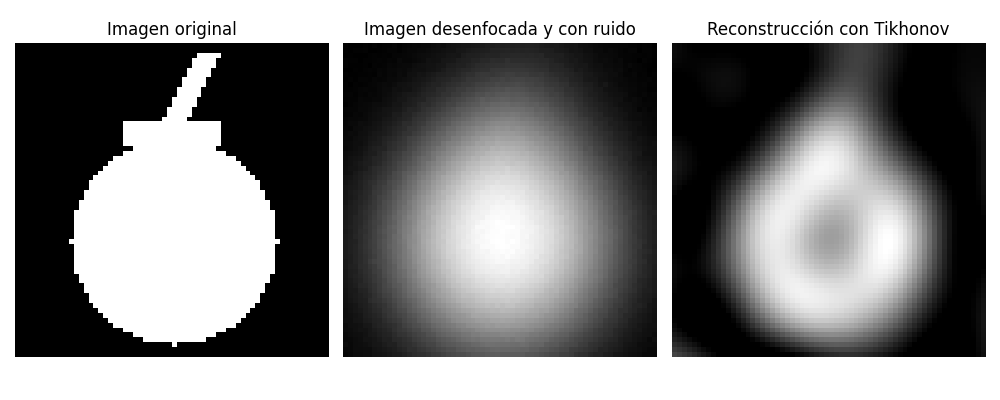
\includegraphics[width=9cm]{Imagenes/Imagenes/mate_tikh.png}
		\end{figure}
		
	\end{frame}
	
	\begin{frame}{Tikhonov Generalizado}
		
		\ Más aún, si utilizamos Tikhonov generalizado $\mathbf{\min_{x} \|Ax-b\|_2^2 + \lambda^2 \|Lx\|_2^2}\,,$ con $L$ el operador de derivada de primer orden, podemos conseguir:
		
		\begin{figure}[htp]
			\centering
			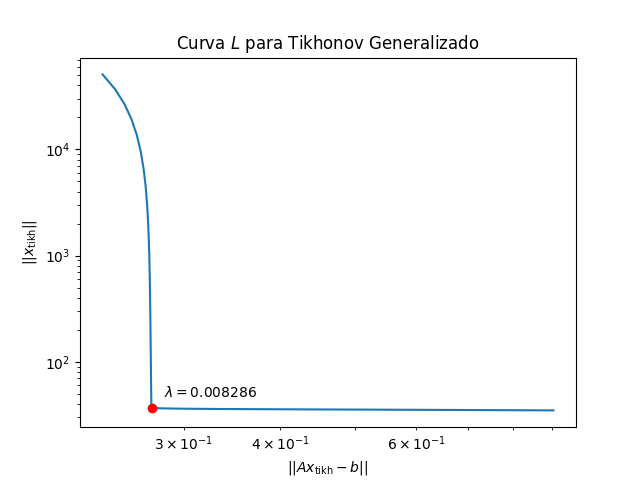
\includegraphics[width=8.5cm]{Imagenes/Imagenes/L_curve_gtikh.png}
		\end{figure}
		
	\end{frame}
	
	\begin{frame}{Tikhonov Generalizado}
		
		\ Y con este $\lambda$ podemos encontrar una pequeña mejora:
		
		\begin{figure}[htp]
			\centering
			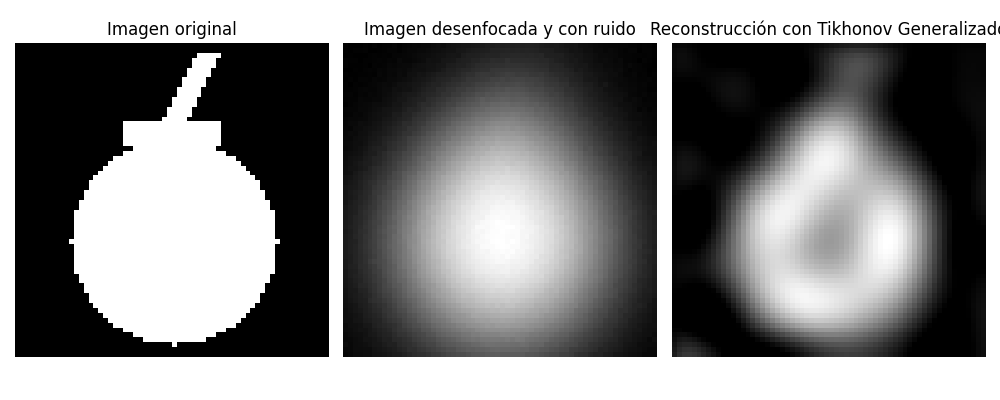
\includegraphics[width=9cm]{Imagenes/Imagenes/mate_gtikh.png}
		\end{figure}
		
	\end{frame}
	
	\begin{frame}{LSQR}
		
		\ Otro enfoque que se le puede dar al problema es usar LSQR para minimizar $\|Ax-b\|_2^2$ a la vez que $\|x\|_2^2$. Aplicandolo obtenemos lo siguiente:
		
		\begin{figure}[htp]
			\centering
			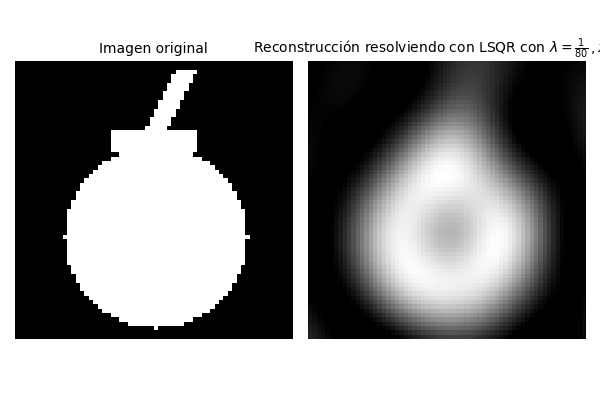
\includegraphics[width=9cm]{Imagenes/Imagenes/mate_lsqr.png}
		\end{figure}
		
	\end{frame}
	
	\begin{frame}{LSMR}
		
		\ De la misma manera, LSMR es un método que también minimiza $\|Ax-b\|_2^2$ a la vez que $\|x\|_2^2$, por lo que resulta en:
		
		\begin{figure}[htp]
			\centering
			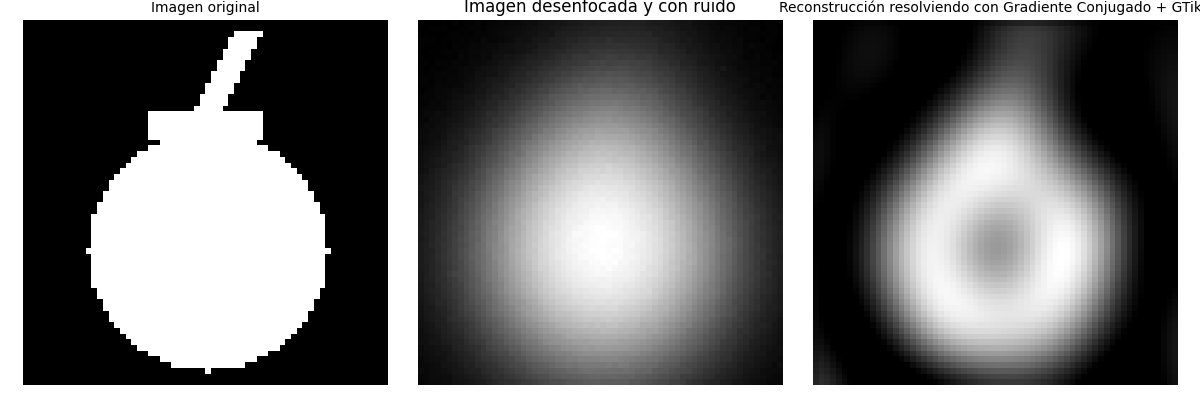
\includegraphics[width=9cm]{Imagenes/Imagenes/mate_lsmr.png}
		\end{figure}
		
	\end{frame}
	
	\begin{frame}{Conclusiones}
		
		\ Como vimos, las maneras de resolver problemas mal condicionados son muchas, todas con distintos requerimientos computacionales y matemáticos. Cada una se puede aplicar de manera satisfactoria dependiendo nuestro problema y las condiciones que tengamos, pero en general siempre hay que hacer un estudio de qué conviene en cada caso.
		
	\end{frame}
	
\end{document}

